\documentclass[12pt]{article}
\usepackage[english]{babel}
\usepackage[utf8x]{inputenc}
\usepackage{amsmath}
\usepackage{graphicx}
\usepackage[colorinlistoftodos]{todonotes}
\usepackage[margin=1in]{geometry}

\begin{document}
	
	\begin{titlepage}
		\newcommand{\HRule}{\noindent\rule{6.5in}{1pt}} % Defines a new command for the horizontal lines, change thickness here
		
		\centering
		
		\textsc{\Large Intro to Artificial Intelligence}\\[.75cm]
		
		\noindent\rule{6.5in}{1.5pt}\\[.75cm]
		{ \huge \bfseries Assignment 1}\\[.4cm]
		{ \large \bfseries Fast Trajectory Planning}\\[.2cm]
		\noindent\rule{6.5in}{1.5pt}\\[1cm]
		
		
		\begin{minipage}{0.4\textwidth}
			\begin{flushleft} \large
				\emph{Authors:}\\
				Brian \textsc{Lin} \\
				Samuel \textsc{Yang}
			\end{flushleft}
		\end{minipage}
		~
		\begin{minipage}{0.4\textwidth}
			\begin{flushright} \large
				\emph{Supervisor:} \\
				Dr.Abdeslam  \textsc{Boularias} % Supervisor's Name
			\end{flushright}
		\end{minipage}\\[2cm]

		
\includegraphics[width=200pt,height=200pt]{RutgersLogo.png}\\[1.5cm]
		\textsc{\Large Rutgers State University of New Jersey}\\[1cm]
		{\large \today}\\[2cm]
		
		\vfill % Fill the rest of the page with whitespace
		
	\end{titlepage}
	
	%\twocolumn
	
	\section*{Introduction}
	
	Your introduction goes here! Some examples of commonly used commands and features are listed below, to help you get started.
	
	If you have a question, please use the support box in the bottom right of the screen to get in touch. 
	\twocolumn
	\section*{Part 1 - Understanding the Methods}
	
	\subsection*{A) - East vs North}
		\begin{figure}[!htb]
			\centering
			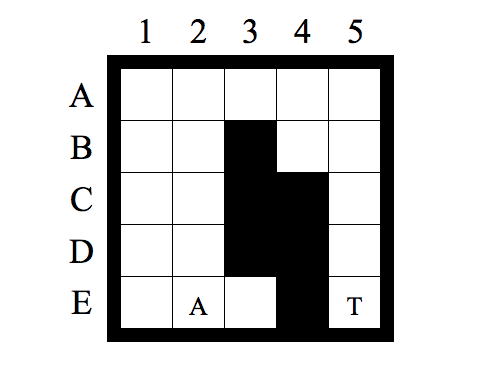
\includegraphics[width=.5\textwidth]{Figure8.png}
			\caption{\label{Figure 8: }Second Example Search Problem}
		\end{figure}
	The agent in the figure above begins it's pathfinding without knowledge of which cells are blocked.  From the perspective of being able to fully observe the maze,
	it appears clear that the best path for the agent is to move north to go around the obstacle.  However, under the initial assumption that all cells are unblocked
	the shortest path from the current cell to the target is to move towards the east, as it has a direct path to the target cell.  Only once the agent has moved to
	the cell to the east, will it observe the blocked cells that do not allow it to use that path and force the agent to find a new path to the target.
	
	\subsection*{B) - Proving Completeness}
	
	\section*{Part 2 - The Effects of Ties}
		\begin{figure}[!htb]
			\centering
			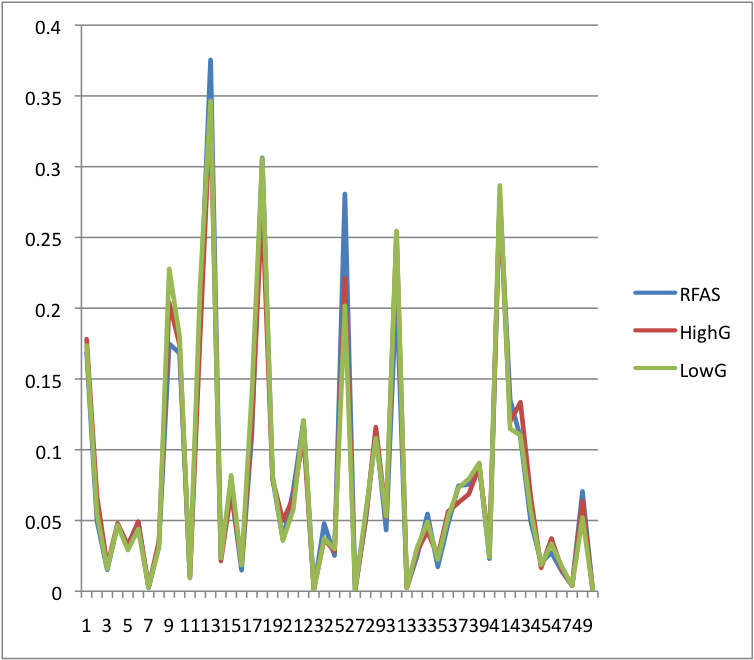
\includegraphics[width=.5\textwidth]{rfas_high_low.png}
			\caption{Effect of g-score based tie-breaking}
		\end{figure}
		The figure above compares the total runtime using 3 different Repeated Forward A* (RFAS) algorithms over 50 test cases. The blue line in the line graph represents the basic RFAS algorithm.  The red line builds on the RFAS by breaking ties between states with the same smallest f-value by choosing the state with the higher g-score.  The green line similarly impacts RFAS by adding in a tiebreaker but instead chooses the state with the lower g-score value.  The data plotted in the figure can be observed in Table 1.  Comparing the total compute times reveals that generally, RFAS implemented with some form of tiebreaker outperformed basic RFAS.  To examine the differences and impact between using based a high g-score or a low g-score on the efficiency of the algorithm, examine Figure 3 and the computational times in Table 1.  
		\begin{figure}[!htb]
			\centering
			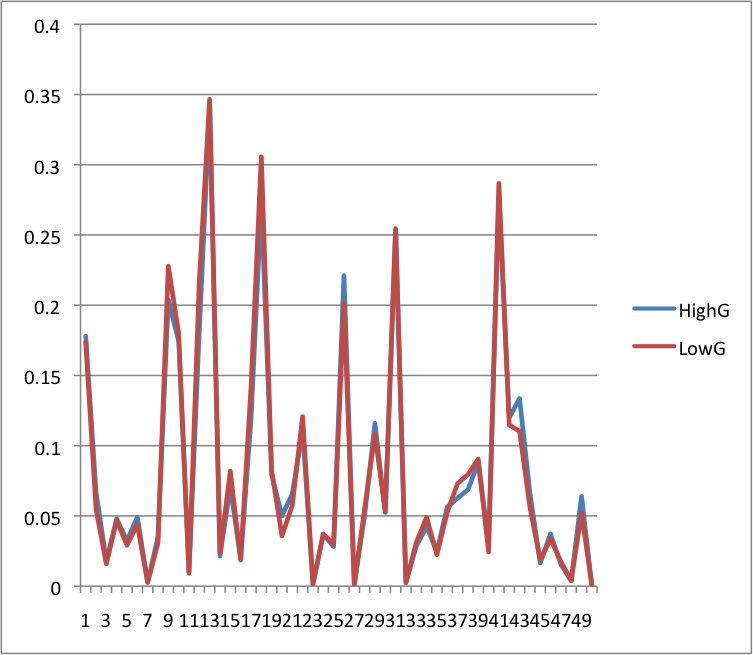
\includegraphics[width=.5\textwidth]{low_high.png}
			\caption{Comparing tie-breaking based on higher g-scores vs lower g-scores}
		\end{figure}
		It is observed that for the majority of test cases, the computational time difference between tiebreakers emphasizing a higher g-score and those that chose a lower g-score were rather small.  However, there is an overall trend of the higher g-score value actually outperforming the lower g-score value that was more observable when the algorithm and the paths were displayed.  To understand the increase in speed and efficiency of the algorithm, recall that the f-score value is a sum of the g-score and the heuristic cost for each cell.  Cells with the same f-score, but having a lower g-score will therefore have a higher heuristic cost, meaning a higher estimate of the moves needed to reach the goal.  Cells with a higher g-score would have a lower heuristic cost and ultimately provide a better path towards the goal cell.  By choosing the higher g-score as a tiebreaker, the agent continues to move towards the target cell while reducing the future distance that would need to be traversed.  
	\section*{Part 3 - Forward vs Backward}
		\begin{figure}[!htb]
			\centering
			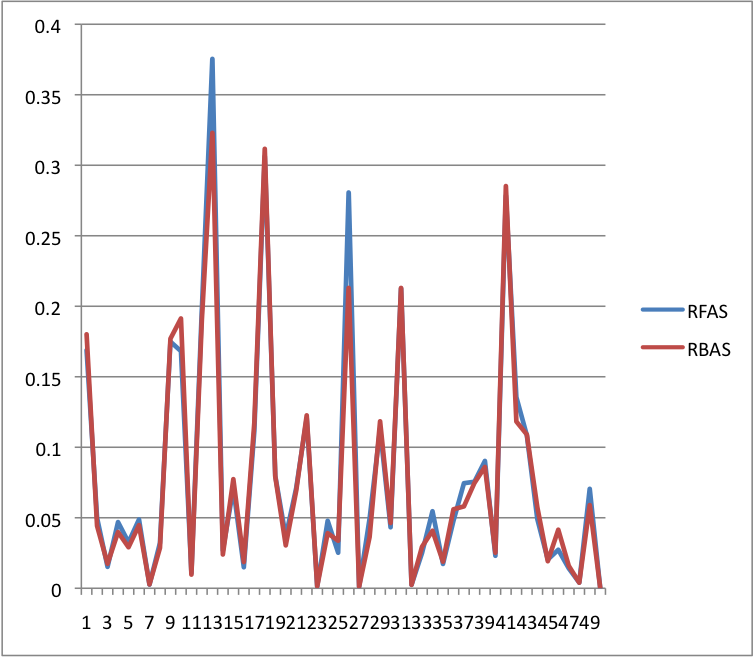
\includegraphics[width=.5\textwidth]{foward_backward.png}
			\caption{Repeated Forward A* vs Repeated Backward A*}
		\end{figure}
		The data represented in the line graph above indicates that again, computational times were incredibly similar.  This time, the comparisons are between Repeated Forward A*, performing the algorithm from the agent cell to the target cell, and Repeated Backward A* (RBAS), having the algorithm traverse the maze from the target cell to the agent.  Examining the data more thoroughly, and observing the displayed output for both instances, it begins to become possible to identify when each algorithm would outperform the other.     
		\onecolumn
		\begin{figure}[!htb]
			\centering
			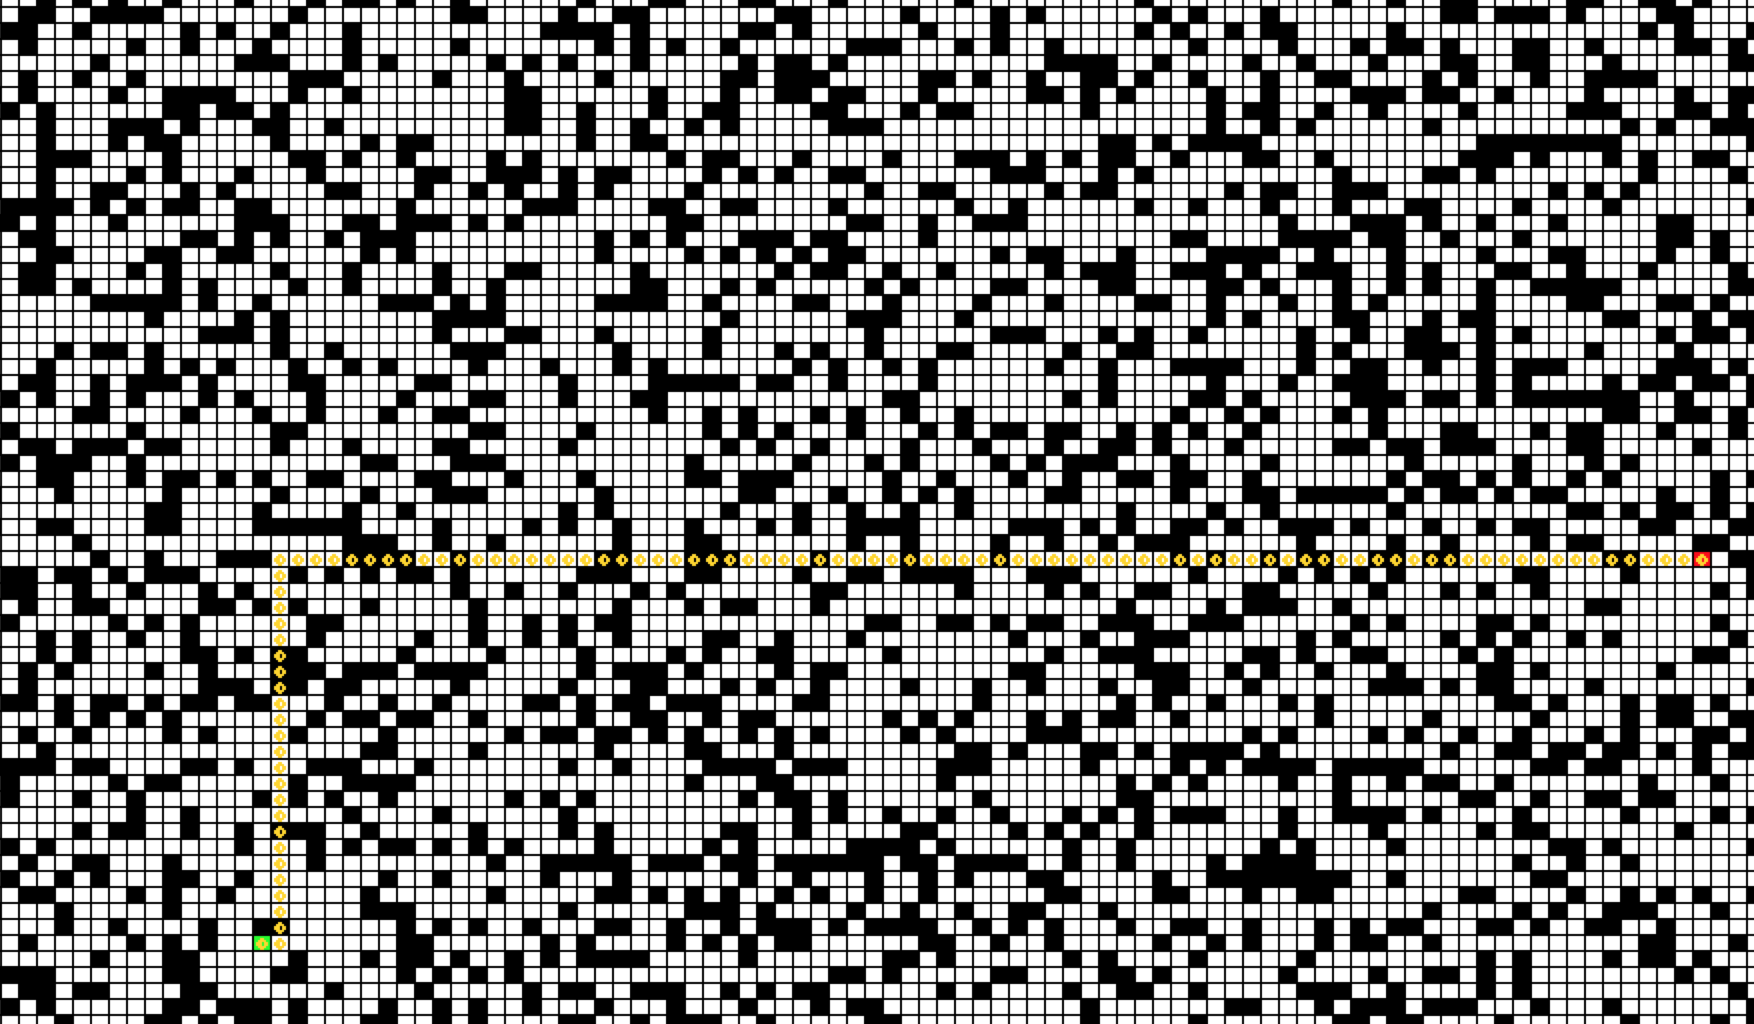
\includegraphics[width=1\textwidth]{test26.png}
			\caption{Test Case 26}
		\end{figure}{1cm}
		In the maze above, the agent cell encounters a heavily blocked off area along its prepared path soon after leaving the initial starting position.  The shape of the blocked cells, rough resembles a wedge, where the agent will move towards the cells at the end of the funnel, as they will have the lowest f-score, but will eventually have to choose a different route as it discovers that there is no viable path through that area.  In this instance, the RBAS algorithm outperformed the RFAS algorithm because when it encounters the blocked off cells that form this trap, it chooses a path that navigates around this obstacle, rather than first exploring it.
		
		In other situations, RFAS is revealed to be the more efficient algorithm than RBAS.  In Figure 6: Test Case 10, found below, one such example can be observed. This time, the target cell has a wedge-like formation of blocked cells that funnels the target cell into more blocked cells until the path would be deemed no longer viable and an alternative one would have to be taken.  
		\twocolumn
		\begin{figure}[!htb]
			\centering
			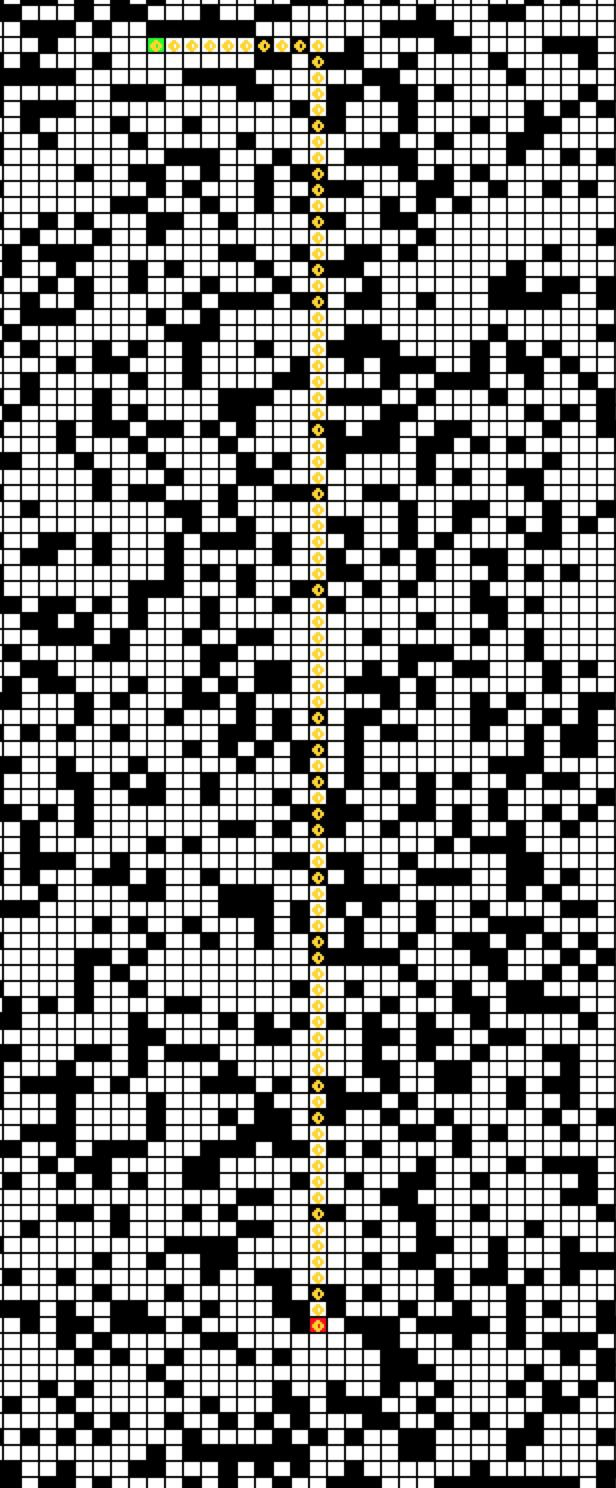
\includegraphics[width=.4\textwidth]{test10.png}
			\caption{Test Case 10}
		\end{figure}  
	
	\section*{Part 4 - Proving Heuristics in the Adaptive A*}
	
		A consistent heuristic function is one where the estimate of a cell will always be less than or equal to the sum of the cost to reach a neighboring cell and the estimated distance from the neighboring cell to the goal.
		
	\section*{Part 5 - Heuristics in the Adaptive A*}
		\begin{figure}[!htb]
			\centering
			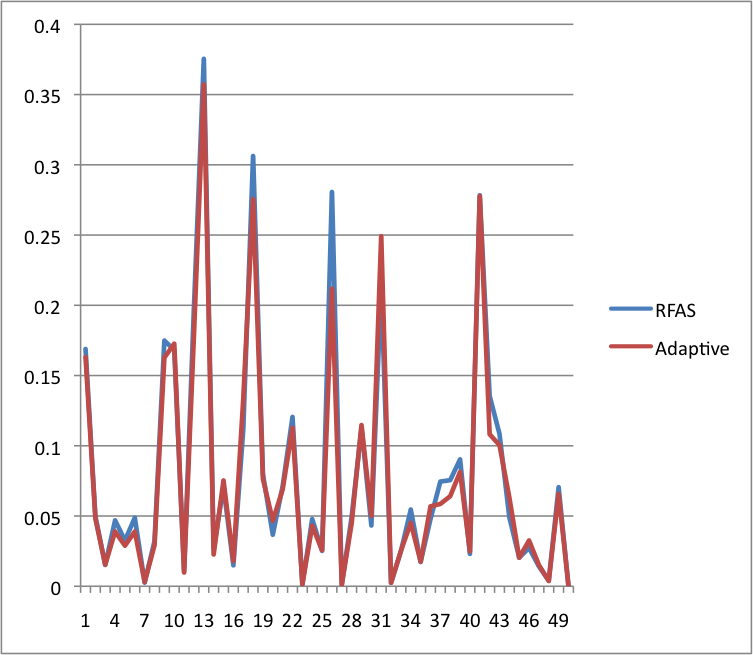
\includegraphics[width=.5\textwidth]{foward_adaptive.png}
			\caption{Comparing RFAS vs Adaptive A*}
		\end{figure}
		The comparison of RFAS and Adaptive A* proved to have the most significant differences in computational times, revealing the observable increase in efficiency that Adaptive A* provides to the algorithm.  During the examination of the various test cases, both algorithms started the initial repetitions at a similar speed.  The speedup became evident as more and more repetitions of A* were computed, as the agent moved away from the initial starting position.  This correlates to the anticipated behavior of Adaptive A* as the implementation of this algorithm means that future A* searches do not have to spend time computing the heuristic costs of previously expanded cells.  Rather, cells that had been expanded in previous iterations would have their heuristics be passed into the current search to reduce the overall computational time.  As the agent moved closer to the target cell, the computational time continued to decrease in comparison to the RFAS.  In all instances where the recorded time of RFAS was faster than the Adaptive A*, the difference was negligible enough that other factors such as processor consistency could account for the time differences.  
	\section*{Part 6 - Memory Issues}
	\onecolumn
	\section*{Recorded Data}
		\begin{table}[!htb]
			\centering
			\begin{tabular}{|c|c|c|c|c|c|}
				Testcase & R.Foward A* &  RFAS HighG & RFAS LowG & R.Backward A* & Adaptive A*\\\hline
				1&0.18031&0.17805&0.17369&0.1801&0.16311\\
				2&0.05316&0.1563&0.05501&0.04421&0.04815\\
				3&0.01451&0.37243&0.01579&0.01735&0.01532\\
				4&0.1154&0.05835&0.04682&0.03984&0.03901\\
				5&0.02399&0.03725&0.02912&0.02909&0.02887\\
				6&0.08087&0.0501&0.04396&0.04474&0.03894\\
				7&0.00426&0.00272&0.00273&0.00274&0.0031\\
				8&0.03738&0.03012&0.03074&0.02859&0.02917\\
				9&0.23135&0.1988&0.22777&0.17702&0.1627\\
				10&0.16354&0.17776&0.18004&0.19133&0.17266\\
				11&0.01025&0.00971&0.00923&0.00969&0.0098\\
				12&0.28907&0.20436&0.21727&0.19082&0.17869\\
				13&0.68515&0.35616&0.34659&0.32296&0.3571\\
				14&0.03878&0.03237&0.02349&0.02396&0.02264\\
				15&0.18915&0.08623&0.08186&0.07736&0.07528\\
				16&0.04573&0.02215&0.01864&0.01861&0.01785\\
				17&0.53899&0.13428&0.14064&0.11699&0.1328\\
				18&0.36806&0.27552&0.30568&0.31164&0.27548\\
				19&0.08804&0.07818&0.08235&0.07921&0.0765\\
				20&0.04013&0.03526&0.03576&0.03042&0.04663\\
				21&0.12534&0.07269&0.05749&0.06926&0.06892\\
				22&0.11665&0.12213&0.12065&0.12261&0.11285\\
				23&0.0022&0.00142&0.0014&0.00141&0.00136\\
				24&0.03575&0.03744&0.03721&0.03908&0.04306\\
				25&0.03671&0.02363&0.02986&0.0337&0.02562\\
			\end{tabular}
		\end{table}
		\begin{table}[!htb]
			\centering
			\begin{tabular}{|c|c|c|c|c|c|}
				Testcase & R.Foward A* &  RFAS HighG & RFAS LowG & R.Backward A* & Adaptive A*\\\hline
				25&0.03671&0.02363&0.02986&0.0337&0.02562\\
				26&0.18862&0.24024&0.20164&0.213&0.21173\\
				27&0.00122&0.00099&0.00111&0.00118&0.00114\\
				28&0.06164&0.05404&0.05515&0.03637&0.04476\\
				29&0.29145&0.12526&0.1081&0.11839&0.11472\\
				30&0.16431&0.04679&0.05303&0.04632&0.05009\\
				31&0.2099&0.23009&0.25453&0.21298&0.24917\\
				32&0.003&0.00245&0.00244&0.00244&0.00246\\
				33&0.03076&0.02806&0.03103&0.02944&0.02524\\
				34&0.04988&0.05898&0.04902&0.04079&0.04513\\
				35&0.02356&0.02285&0.02236&0.01885&0.01753\\
				36&0.18883&0.06269&0.0526&0.056&0.05686\\
				37&0.03722&0.05894&0.07305&0.05806&0.0586\\
				38&0.13161&0.07622&0.07941&0.07465&0.06411\\
				39&0.09456&0.09503&0.09055&0.08602&0.08135\\
				40&0.06185&0.02452&0.02434&0.02521&0.0249\\
				41&0.53071&0.28605&0.28678&0.28523&0.27768\\
				42&0.20066&0.13528&0.11477&0.11826&0.1082\\
				43&0.7402&0.10712&0.11034&0.10902&0.10043\\
				44&0.09136&0.05433&0.05641&0.05744&0.06319\\
				45&0.02809&0.01911&0.01862&0.01919&0.02032\\
				46&0.063&0.03151&0.03352&0.04151&0.03259\\
				47&0.01576&0.01462&0.01756&0.01589&0.01512\\
				48&0.0051&0.00394&0.00393&0.00397&0.00373\\
				49&0.09776&0.07013&0.05215&0.05897&0.06572\\
				50&0.0003&0.00025&0.00039&0.00031&0.00023\\
			\end{tabular}
			\caption{\label{tab:widgets}An example table.}
		\end{table}
	\iffalse
		\section{Some \LaTeX{} Examples}
		\label{sec:examples}
		
		\subsection{Sections}
		
		Use section and subsection commands to organize your document. \LaTeX{} handles all the formatting and numbering automatically. Use ref and label commands for cross-references.
		
		\subsection{Comments}
		
		Comments can be added to the margins of the document using the \todo{Here's a comment in the margin!} todo command, as shown in the example on the right. You can also add inline comments too:
		
		\todo[inline, color=green!40]{This is an inline comment.}
		
		\subsection{Tables and Figures}
		
		Use the table and tabular commands for basic tables --- see Table~\ref{tab:widgets}, for example. You can upload a figure (JPEG, PNG or PDF) using the files menu. To include it in your document, use the includegraphics command as in the code for Figure~\ref{fig:frog} below.
		
		% Commands to include a figure:
		%\begin{figure}
		%	\centering
			%\includegraphics[width=0.5\textwidth]{frog.jpg}
		%	\caption{\label{fig:frog}This is a figure caption.}
		%\end{figure}
		
		%\begin{table}
		%%	\begin{tabular}{l|r}
				%Item & Quantity \\\hline
				%Widgets & 42 \\
				%Gadgets & 13
		%	\end{tabular}
		%	\caption{\label{tab:widgets}An example table.}
		%\end{table}
		
		\subsection{Mathematics}
		
		\LaTeX{} is great at typesetting mathematics. Let $X_1, X_2, \ldots, X_n$ be a sequence of independent and identically distributed random variables with $\text{E}[X_i] = \mu$ and $\text{Var}[X_i] = \sigma^2 < \infty$, and let
		$$S_n = \frac{X_1 + X_2 + \cdots + X_n}{n}
		= \frac{1}{n}\sum_{i}^{n} X_i$$
		denote their mean. Then as $n$ approaches infinity, the random variables $\sqrt{n}(S_n - \mu)$ converge in distribution to a normal $\mathcal{N}(0, \sigma^2)$.
		
		\subsection{Lists}
		
		You can make lists with automatic numbering \dots
		
		\begin{enumerate}
			\item Like this,
			\item and like this.
		\end{enumerate}
		\dots or bullet points \dots
		\begin{itemize}
			\item Like this,
			\item and like this.
		\end{itemize}
	\fi
	
\end{document}